\chapter{Paper I:\@
  Mechanism of \ce{Pd(II)}-mediated\linebreak uncaging reactions % chktex 36
  of propargylic substrates
 }%
\label{ch:paper1}

\fullcite{Coelho_2019}

% Abstract
Palladium-catalysed chemical uncaging of propargylic substrates involves C–O bond breaking and is inhibited by product.
Biphasic kinetics of C–O bond breaking through anti-Markovnikov hydration and β-O elimination and Pd(0) hydrolysis are described.

% Introduction
Pd-mediated C–O bond cleavage is a strategy for bioorthogonal uncaging of protected molecules under biocompatible conditions.
Design must consider catalyst solubility and toxicity for efficient uncaging reactions.
Investigation of the bond-cleavage of propargyl-protected hydroxyl groups from prodrug compound DNPPE using Pd(II) salts in phosphate-buffered aqueous medium.

% Results and discussion
Pd(II) salts mediated reactions monitored by UV-vis spectroscopy, deviating from first-order kinetics, typical of biphasic kinetics with two observed macroscopic rate constants (k1, k2).
The two reaction kinetics profiles, Rx1 (15 times faster than Rx2) and Rx2, have half lifes of ∼1 h and ∼650 times faster than the uncatalyzed reaction.
Rx1 is responsible for two turnovers of ∼20mol\% product, while Rx2 has sharp increase after two turnovers.
RPKA suggests catalyst deactivation and product inhibition, but experiments showed that neither was likely to be happening.
Reaction rates changed significantly with changes in Pd concentration, buffer and cosolvent, suggesting different catalyst nuclearities and complexation interactions.
No Pd(0) was spontaneously formed during a 3-hour XAS experiment without addition of substrate.
The two mechanistic scenarios involve a Pd(0) or a Pd(II) reaction, but experiments showed Pd(0) does not participate in the faster phase.
ESI-HRMS used to detect key reaction intermediates in Pd catalysed reaction.
Ion 3 was characterized by ESI–CID–MS/MS as a hydrolyzed carbopalladate intermediate complexed with another DNPPE molecule.
Kinetic studies and XAS results indicate alkyne hydration as initial part of reaction, with computational studies performed to investigate.
Both anti-Markovnikov and Markovnikov keto intermediates undergo β-O elimination and SN2-like hydrolysis, but Markovnikov is significantly less favorable.
Rx1 involves Pd(II) coordination, anti-Markovnikov attack, C-O bond breaking and hydration, with final products of two equivalents of DNP and the carbopalladate complex 8.
Insertion of propargyl ether facilitates hydration of triplet bond and stabilizes keto intermediate in C–O bond breaking.
Propargyl alcohol inhibited further complexation, confirming the proposed mechanism for Rx1.
The reaction produced Pd nanoparticles and mixed palladium oxidation states.
The addition of CS2 completely inhibited Rx2 catalytic activity and Hg(0) inhibited it by ∼60\%, indicating the activity of Pd(0) NPs or lixiviated Pd(0) atoms.
Two different catalytic cycles convert two equivalents of substrate in the DNPPE O-depropargylation reaction catalyzed by Pd(II).

% Conclusions
Pd(II) salts act as catalysts for O-depropargylation with two phases, one fast and one slow due to product inhibition, creating a need for high catalysts doses.
Products may be tuned by bulky ligands to prevent catalysts inhibition.

MY TEXT BELOW

In order to develop better \ce{C-O} bond cleavage promoters,
recently, bioorthogonal approaches have been devised to promote \ce{C-O} bond
cleavage by trainsition metals for uncaging protected molecules, normally with
hydroxyl and amino functional groups.
Palladium (II) has been extensively used for such biocompatible processes.
Uncaging of propargyl groups has remained challenging.
This reaction has been added to the bioorthogonal arsenal of chemical biology and
medicional chemistry for activating bio and prodrug molecules recently.

It is normally assumed that the process goes through \emph{in situ} formation
of catalytic \ce{Pd(0)}, promoted by a base through intramolecular ligand exchange
reduction or nucleophilic attack by the solvent and then suffering reductive
elimination.
This \ce{Pd(0)} could then undergo oxidative addition with the
propargyl group, producing an allenylpalladium intermediate, which is then
hydrolyzed, regenerating the \ce{Pd(0)} and producing acetol as the side product.
A less common hypothetical alternative is the \ce{Pd(II)}-mediated hydration
mechanism to form an intermediate that then decomposes by hydrolisys
(Wacker-like oxidation WHAT IS THIS).

In this work, we attempted to unveil through which mechanism does
the Palladium(II)-mediated chemical uncaging reaction of
progargyl-protected hydroxyl groups takes place.
The reactions were monitored in the lab by UV-vis spectroscopy and a deviation
from first-order kinetics was observed.
A distinct biexponential shape was found, consistent with biphasic kinetics,
which produce the same product (DNP) at different reaction rates.
The fastest reaction has a half-life or 1 hour, and was found to be around 15 times faster than the other, and
650 times faster than the uncatalyzed one.

It was observed that the fast phase was responsible for only two turnovers,
which indicates that, although faster, it shuts down after two turnovers.
Further experiments evidenced that the catalyst may not be stable and is changing through the
course of the reaction, changing its activity.
Furthermore, neither DNP or acetol seem to inhibit the reaction.

With the XAS results, we proceeded to perform computational studies.
We employed the \ce{[PdCl4]2-} complex as the catalyst species, and chose a
model substrate methylpropargyl ether to simplify calculations.
We employed an implicit solvation model in water, and used two explicit extra
water molecules to consider the effect of hydrogen bonding, one interacting
with the enol part and the other with the leaving group.
We used PBE0 to obtain geometries and frequencies, and adjusted the electronic
energy with DLPNO-CCSD(T) and HF-gCP to correct for basis set artifacts.

We found out that both Markovnikov and anti-Markovnikov regiochemical
hydrations of the Pd-propargyl complex to form enols are competitive and within
the method's error (< 1~\kcalmol).
% TODO: CONTINUE FROM THE PARAGRAPH BEFORE FIGURE 4.

Our evidence suggested that the reaction proceeds through biphasic kinetics
with different rates, where the most favorable path involves a \ce{Pd(II)}
anti-Markovnikov hydration of the propargyl group, followed by C-O bond breaking
by $\beta$-O elimination.
The process lasts two turnovers as the product inhibits further
reactivity.

An application to metallocatalysis~\cite{Coelho_2019}.
A computational-experimental collaboration.

% TODO: WHICH SUBSTRATES WE USED, RELATE TO COMPUTATION\@?

\section{Paper}

The publication can be read in full next.

Reprinted with permission from
\fullcite{Coelho_2019}.
Copyright
\citeyear{Coelho_2019}
American~Chemical~Society.

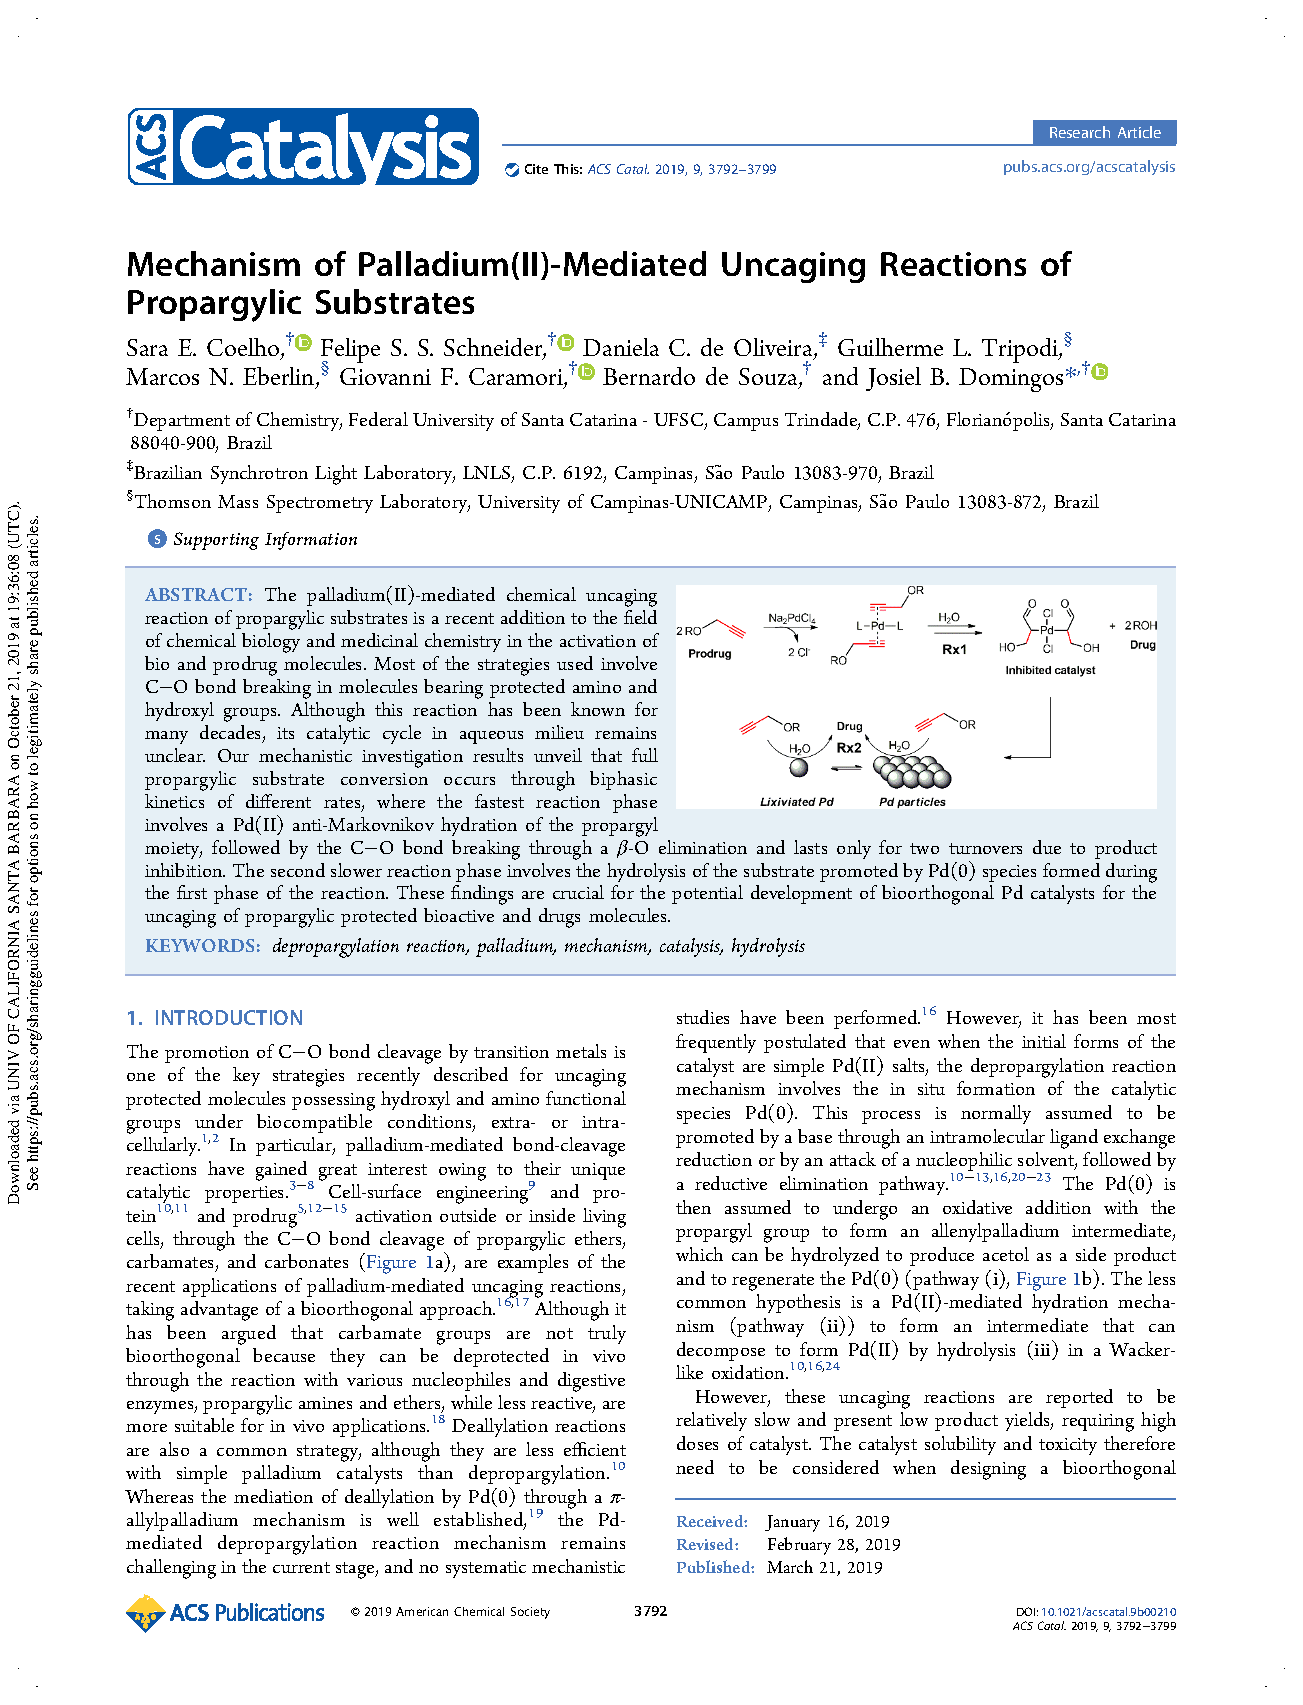
\includepdf[pages=-]{pubs/coelho2019-paper1.pdf}
